
        \documentclass[spanish, 11pt]{exam}

        %These tell TeX which packages to use.
        \usepackage{array,epsfig}
        \usepackage{amsmath, textcomp}
        \usepackage{amsfonts}
        \usepackage{amssymb}
        \usepackage{amsxtra}
        \usepackage{amsthm}
        \usepackage{mathrsfs}
        \usepackage{color}
        \usepackage{multicol, xparse}
        \usepackage{verbatim}


        \usepackage[utf8]{inputenc}
        \usepackage[spanish]{babel}
        \usepackage{eurosym}

        \usepackage{graphicx}
        \graphicspath{{../img/}}
        \usepackage{pgf}



        \printanswers
        \nopointsinmargin
        \pointformat{}

        %Pagination stuff.
        %\setlength{\topmargin}{-.3 in}
        %\setlength{\oddsidemargin}{0in}
        %\setlength{\evensidemargin}{0in}
        %\setlength{\textheight}{9.in}
        %\setlength{\textwidth}{6.5in}
        %\pagestyle{empty}

        \let\multicolmulticols\multicols
        \let\endmulticolmulticols\endmulticols
        \RenewDocumentEnvironment{multicols}{mO{}}
         {%
          \ifnum#1=1
            #2%
          \else % More than 1 column
            \multicolmulticols{#1}[#2]
          \fi
         }
         {%
          \ifnum#1=1
          \else % More than 1 column
            \endmulticolmulticols
          \fi
         }
        \renewcommand{\solutiontitle}{\noindent\textbf{Sol:}\enspace}

        \newcommand{\samedir}{\mathbin{\!/\mkern-5mu/\!}}

        \newcommand{\class}{1º Bachillerato}
        \newcommand{\examdate}{\today}

        \newcommand{\tipo}{A}


        \newcommand{\timelimit}{50 minutos}



        \pagestyle{head}
        \firstpageheader{
\includegraphics[width=0.2\columnwidth]{header_left}}{\textbf{Departamento de Matemáticas\linebreak \class}\linebreak \examnum}{
\includegraphics[width=0.1\columnwidth]{header_right}}
        \runningheader{\class}{\examnum}{Página \thepage\ of \numpages}
        \runningheadrule

        \newcommand{\examnum}{Autoevaluación de Estadística}
        \begin{document}
        \begin{questions}
        \question au0pe02 - Se realiza una encuesta a un grupo de 21 personas acerca del número de veces que acuden al cine a lo largo de un año, obteniéndose los siguientes resultados:4 2 6 8 3 4 3 5 7 1 3 4 5 7 2 2 1 3 12 5 4
        \begin{multicols}{1}
        \begin{parts} \part[1] Realiza una tabla de frecuencias  \begin{solution}   \begin{tabular}{rrrrrrr}
\hline
   x\_i &   f\_i &   F\_i &       h\_i &       H\_i &      \%\_i &      \%A\_i \\
\hline
     1 &     2 &     2 & 0.0952381 & 0.0952381 &  9.52381 &   9.52381 \\
     2 &     3 &     5 & 0.142857  & 0.238095  & 14.2857  &  23.8095  \\
     3 &     4 &     9 & 0.190476  & 0.428571  & 19.0476  &  42.8571  \\
     4 &     4 &    13 & 0.190476  & 0.619048  & 19.0476  &  61.9048  \\
     5 &     3 &    16 & 0.142857  & 0.761905  & 14.2857  &  76.1905  \\
     6 &     1 &    17 & 0.047619  & 0.809524  &  4.7619  &  80.9524  \\
     7 &     2 &    19 & 0.0952381 & 0.904762  &  9.52381 &  90.4762  \\
     8 &     1 &    20 & 0.047619  & 0.952381  &  4.7619  &  95.2381  \\
    12 &     1 &    21 & 0.047619  & 1         &  4.7619  & 100       \\
\hline
\end{tabular}   \end{solution} \part[1] Realiza un diagrama de barras y un polígono de frecuencias  \begin{solution}   \\ \resizebox {0.5\textwidth}{!}{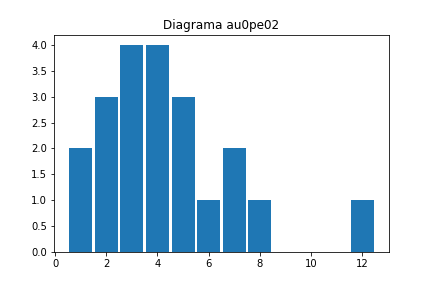
\includegraphics[width=1\columnwidth]{au0pe02}}   \end{solution} \part[1] Calcular los parámetros de centralización  \begin{solution}   {'media': 4.333333333333333, 'mediana': 4.0, 'moda': ModeResult(mode=array([3]), count=array([4]))}   \end{solution} \part[1] Calcular los parámetros de posición P70, Q1, Q3, D4  \begin{solution}   {'P70': 5.0, 'Q1': 3.0, 'Q3': 5.0, 'D4': 3.0}   \end{solution} \part[1] Calcular los parámetros de dispersión  \begin{solution}   {'rango': 11, 'varianza': 6.507936507936508, 'desviación típica': 2.55106575923407, 'coeficiente variación': 0.588707482900170}   \end{solution}
        \end{parts}
        \end{multicols}
        \question au1p090e06 - La medida del tórax de una muestra de varones se distribuye: \\\begin{tabular}{rlr}
\hline
    & Duración                    &   Cantidad \\
\hline
  0 & $\left[79.5, 85.5\right)$   &          4 \\
  1 & $\left[85.5, 91.5\right)$   &          8 \\
  2 & $\left[91.5, 97.5\right)$   &         12 \\
  3 & $\left[97.5, 103.5\right)$  &         20 \\
  4 & $\left[103.5, 109.5\right)$ &          9 \\
  5 & $\left[109.5, 115.5\right)$ &          5 \\
  6 & $\left[115.5, 121.5\right)$ &          2 \\
\hline
\end{tabular}
        \begin{multicols}{1}
        \begin{parts} \part[1] Haz una tabla de frecuencias  \begin{solution}   \begin{tabular}{rrrrrrrrrr}
\hline
    &   lim\_inf &   lim\_sup &   x\_i &   f\_i &   F\_i &       h\_i &         H\_i &   x\_if\_i &   x\^{}2\_if\_i \\
\hline
  0 &      79.5 &      85.5 &  82.5 &     4 &     4 & 0.0666667 &   0.0666667 &    330   &    27225   \\
  1 &      85.5 &      91.5 &  88.5 &     8 &    12 & 0.133333  &   0.2       &    708   &    62658   \\
  2 &      91.5 &      97.5 &  94.5 &    12 &    24 & 0.2       &   0.4       &   1134   &   107163   \\
  3 &      97.5 &     103.5 & 100.5 &    20 &    44 & 0.333333  &   0.733333  &   2010   &   202005   \\
  4 &     103.5 &     109.5 & 106.5 &     9 &    53 & 0.15      &   0.883333  &    958.5 &   102080   \\
  5 &     109.5 &     115.5 & 112.5 &     5 &    58 & 0.0833333 &   0.966667  &    562.5 &    63281.2 \\
  6 &     115.5 &     121.5 & 118.5 &     2 &    60 & 0.0333333 &   1         &    237   &    28084.5 \\
  7 &     nan   &     nan   & nan   &    60 &   nan & 1         & nan         &   5940   &   592497   \\
\hline
\end{tabular}   \end{solution} \part[1] Calcula media, la varianza, la desviación típica y el coeficiente de variación  \begin{solution}   {'media': 99.0, 'varianza': 73.95000000000073, 'desviación típica': 8.59941858499752, 'coeficiente de variación': 0.0868628139898739}   \end{solution}
        \end{parts}
        \end{multicols}
        \question au2p090e07 - En una consulta médica la distribución de pacientes por su edad ha sido, en la última semana, la siguiente:\\\begin{tabular}{rlr}
\hline
    & Duración              &   Cantidad \\
\hline
  0 & $\left[15, 23\right)$ &          3 \\
  1 & $\left[23, 31\right)$ &          4 \\
  2 & $\left[31, 39\right)$ &          5 \\
  3 & $\left[39, 47\right)$ &          8 \\
  4 & $\left[47, 55\right)$ &         10 \\
  5 & $\left[55, 63\right)$ &         12 \\
  6 & $\left[63, 71\right)$ &         15 \\
  7 & $\left[71, 79\right)$ &         12 \\
  8 & $\left[79, 87\right)$ &          6 \\
\hline
\end{tabular}
        \begin{multicols}{1}
        \begin{parts} \part[1] Haz una tabla de frecuencias  \begin{solution}   \begin{tabular}{rrrrrrrrrr}
\hline
    &   lim\_inf &   lim\_sup &   x\_i &   f\_i &   F\_i &       h\_i &         H\_i &   x\_if\_i &   x\^{}2\_if\_i \\
\hline
  0 &        15 &        23 &    19 &     3 &     3 & 0.04      &   0.04      &       57 &       1083 \\
  1 &        23 &        31 &    27 &     4 &     7 & 0.0533333 &   0.0933333 &      108 &       2916 \\
  2 &        31 &        39 &    35 &     5 &    12 & 0.0666667 &   0.16      &      175 &       6125 \\
  3 &        39 &        47 &    43 &     8 &    20 & 0.106667  &   0.266667  &      344 &      14792 \\
  4 &        47 &        55 &    51 &    10 &    30 & 0.133333  &   0.4       &      510 &      26010 \\
  5 &        55 &        63 &    59 &    12 &    42 & 0.16      &   0.56      &      708 &      41772 \\
  6 &        63 &        71 &    67 &    15 &    57 & 0.2       &   0.76      &     1005 &      67335 \\
  7 &        71 &        79 &    75 &    12 &    69 & 0.16      &   0.92      &      900 &      67500 \\
  8 &        79 &        87 &    83 &     6 &    75 & 0.08      &   1         &      498 &      41334 \\
  9 &       nan &       nan &   nan &    75 &   nan & 1         & nan         &     4305 &     268867 \\
\hline
\end{tabular}   \end{solution} \part[1] Calcula media, la varianza, la desviación típica y el coeficiente de variación  \begin{solution}   {'media': 57.4, 'varianza': 290.13333333333367, 'desviación típica': 17.0333007175161, 'coeficiente de variación': 0.296747399259862}   \end{solution} \part[1] La edad mas frecuente de los pacientes  \begin{solution}   {'Intervalo modal': '$\\left[63.0, 71.0\\right)$', 'moda': 67.0}   \end{solution} \part[1] El percentil 47  \begin{solution}   {'k': 47, 'N': 75.0, '$L_i$': 55.0, '$f_i$': 12.0, '$F_{i-1}$': 30.0, '$C_i$': 8.0, 'percentil': 58.5}   \end{solution} \part[1] ¿Qué porcentaje de pacientes tenían una edad superior a 60 años?  \begin{solution}   {'valor': 60, 'N': 75.0, '$L_i$': 55.0, '$f_i$': 12.0, '$F_{i-1}$': 30.0, '$C_i$': 8.0, 'Porcentaje': 50.0000000000000}   \end{solution}
        \end{parts}
        \end{multicols}
        \question au3p093e05 - La temperatura media en los meses de invierno en varias ciudades y el gasto medio por habitante en
calefacción ha sido\\\begin{tabular}{lrrrrrr}
\hline
                      &   0 &   1 &   2 &   3 &   4 &   5 \\
\hline
 Temperatura (grados) &  10 &  12 &  14 &  15 &  17 &  20 \\
 Gasto (euros)        & 150 & 120 & 102 &  90 &  50 &  18 \\
\hline
\end{tabular}
        \begin{multicols}{1}
        \begin{parts} \part[1] Haz una tabla de frecuencias con los datos que necesites para hace el resto de apartados  \begin{solution}   \begin{tabular}{rrrrrr}
\hline
    &   x &   y &   xy &   x2 &    y2 \\
\hline
  0 &  10 & 150 & 1500 &  100 & 22500 \\
  1 &  12 & 120 & 1440 &  144 & 14400 \\
  2 &  14 & 102 & 1428 &  196 & 10404 \\
  3 &  15 &  90 & 1350 &  225 &  8100 \\
  4 &  17 &  50 &  850 &  289 &  2500 \\
  5 &  20 &  18 &  360 &  400 &   324 \\
  6 &  88 & 530 & 6928 & 1354 & 58228 \\
\hline
\end{tabular}   \end{solution} \part[1] Calcula el gasto medio  \begin{solution}   {'media': 88.33333333333333}   \end{solution} \part[1] Halla el coeficiente de correlación lineal e interprétalo  \begin{solution}   {'media de x': 14.666666666666666, 'desviación de x': 3.2489314482696545, 'media de y': 88.33333333333333, 'desviación de y': 43.61065109453067, 'covarianza': -140.88888888888889, 'coeficiente de correlación': -0.9943599539663297}   \end{solution} \part[1] Estima el gasto medio por habitante de una ciudad si la temperatura media hubiera sido 8ºC  \begin{solution}   $y = - 13.3473684210526 x + 284.094736842105$ \\\resizebox {0.5\textwidth}{!}{%% Creator: Matplotlib, PGF backend
%%
%% To include the figure in your LaTeX document, write
%%   \input{<filename>.pgf}
%%
%% Make sure the required packages are loaded in your preamble
%%   \usepackage{pgf}
%%
%% Figures using additional raster images can only be included by \input if
%% they are in the same directory as the main LaTeX file. For loading figures
%% from other directories you can use the `import` package
%%   \usepackage{import}
%% and then include the figures with
%%   \import{<path to file>}{<filename>.pgf}
%%
%% Matplotlib used the following preamble
%%   \usepackage{fontspec}
%%   \setmainfont{DejaVuSerif.ttf}[Path=/home/hp/Mis_aplicaciones/anaconda3/lib/python3.6/site-packages/matplotlib/mpl-data/fonts/ttf/]
%%   \setsansfont{DejaVuSans.ttf}[Path=/home/hp/Mis_aplicaciones/anaconda3/lib/python3.6/site-packages/matplotlib/mpl-data/fonts/ttf/]
%%   \setmonofont{DejaVuSansMono.ttf}[Path=/home/hp/Mis_aplicaciones/anaconda3/lib/python3.6/site-packages/matplotlib/mpl-data/fonts/ttf/]
%%
\begingroup%
\makeatletter%
\begin{pgfpicture}%
\pgfpathrectangle{\pgfpointorigin}{\pgfqpoint{6.000000in}{4.000000in}}%
\pgfusepath{use as bounding box, clip}%
\begin{pgfscope}%
\pgfsetbuttcap%
\pgfsetmiterjoin%
\definecolor{currentfill}{rgb}{1.000000,1.000000,1.000000}%
\pgfsetfillcolor{currentfill}%
\pgfsetlinewidth{0.000000pt}%
\definecolor{currentstroke}{rgb}{1.000000,1.000000,1.000000}%
\pgfsetstrokecolor{currentstroke}%
\pgfsetdash{}{0pt}%
\pgfpathmoveto{\pgfqpoint{0.000000in}{0.000000in}}%
\pgfpathlineto{\pgfqpoint{6.000000in}{0.000000in}}%
\pgfpathlineto{\pgfqpoint{6.000000in}{4.000000in}}%
\pgfpathlineto{\pgfqpoint{0.000000in}{4.000000in}}%
\pgfpathclose%
\pgfusepath{fill}%
\end{pgfscope}%
\begin{pgfscope}%
\pgfsetbuttcap%
\pgfsetmiterjoin%
\definecolor{currentfill}{rgb}{1.000000,1.000000,1.000000}%
\pgfsetfillcolor{currentfill}%
\pgfsetlinewidth{0.000000pt}%
\definecolor{currentstroke}{rgb}{0.000000,0.000000,0.000000}%
\pgfsetstrokecolor{currentstroke}%
\pgfsetstrokeopacity{0.000000}%
\pgfsetdash{}{0pt}%
\pgfpathmoveto{\pgfqpoint{0.750000in}{0.500000in}}%
\pgfpathlineto{\pgfqpoint{5.400000in}{0.500000in}}%
\pgfpathlineto{\pgfqpoint{5.400000in}{3.520000in}}%
\pgfpathlineto{\pgfqpoint{0.750000in}{3.520000in}}%
\pgfpathclose%
\pgfusepath{fill}%
\end{pgfscope}%
\begin{pgfscope}%
\pgfpathrectangle{\pgfqpoint{0.750000in}{0.500000in}}{\pgfqpoint{4.650000in}{3.020000in}}%
\pgfusepath{clip}%
\pgfsetbuttcap%
\pgfsetroundjoin%
\definecolor{currentfill}{rgb}{0.121569,0.466667,0.705882}%
\pgfsetfillcolor{currentfill}%
\pgfsetfillopacity{0.800000}%
\pgfsetlinewidth{1.003750pt}%
\definecolor{currentstroke}{rgb}{0.121569,0.466667,0.705882}%
\pgfsetstrokecolor{currentstroke}%
\pgfsetstrokeopacity{0.800000}%
\pgfsetdash{}{0pt}%
\pgfpathmoveto{\pgfqpoint{0.967457in}{3.049833in}}%
\pgfpathcurveto{\pgfqpoint{0.978507in}{3.049833in}}{\pgfqpoint{0.989106in}{3.054223in}}{\pgfqpoint{0.996920in}{3.062037in}}%
\pgfpathcurveto{\pgfqpoint{1.004734in}{3.069850in}}{\pgfqpoint{1.009124in}{3.080449in}}{\pgfqpoint{1.009124in}{3.091500in}}%
\pgfpathcurveto{\pgfqpoint{1.009124in}{3.102550in}}{\pgfqpoint{1.004734in}{3.113149in}}{\pgfqpoint{0.996920in}{3.120962in}}%
\pgfpathcurveto{\pgfqpoint{0.989106in}{3.128776in}}{\pgfqpoint{0.978507in}{3.133166in}}{\pgfqpoint{0.967457in}{3.133166in}}%
\pgfpathcurveto{\pgfqpoint{0.956407in}{3.133166in}}{\pgfqpoint{0.945808in}{3.128776in}}{\pgfqpoint{0.937994in}{3.120962in}}%
\pgfpathcurveto{\pgfqpoint{0.930181in}{3.113149in}}{\pgfqpoint{0.925790in}{3.102550in}}{\pgfqpoint{0.925790in}{3.091500in}}%
\pgfpathcurveto{\pgfqpoint{0.925790in}{3.080449in}}{\pgfqpoint{0.930181in}{3.069850in}}{\pgfqpoint{0.937994in}{3.062037in}}%
\pgfpathcurveto{\pgfqpoint{0.945808in}{3.054223in}}{\pgfqpoint{0.956407in}{3.049833in}}{\pgfqpoint{0.967457in}{3.049833in}}%
\pgfpathclose%
\pgfusepath{stroke,fill}%
\end{pgfscope}%
\begin{pgfscope}%
\pgfpathrectangle{\pgfqpoint{0.750000in}{0.500000in}}{\pgfqpoint{4.650000in}{3.020000in}}%
\pgfusepath{clip}%
\pgfsetbuttcap%
\pgfsetroundjoin%
\definecolor{currentfill}{rgb}{0.121569,0.466667,0.705882}%
\pgfsetfillcolor{currentfill}%
\pgfsetfillopacity{0.800000}%
\pgfsetlinewidth{1.003750pt}%
\definecolor{currentstroke}{rgb}{0.121569,0.466667,0.705882}%
\pgfsetstrokecolor{currentstroke}%
\pgfsetstrokeopacity{0.800000}%
\pgfsetdash{}{0pt}%
\pgfpathmoveto{\pgfqpoint{1.810474in}{2.558223in}}%
\pgfpathcurveto{\pgfqpoint{1.821524in}{2.558223in}}{\pgfqpoint{1.832123in}{2.562613in}}{\pgfqpoint{1.839937in}{2.570427in}}%
\pgfpathcurveto{\pgfqpoint{1.847751in}{2.578241in}}{\pgfqpoint{1.852141in}{2.588840in}}{\pgfqpoint{1.852141in}{2.599890in}}%
\pgfpathcurveto{\pgfqpoint{1.852141in}{2.610940in}}{\pgfqpoint{1.847751in}{2.621539in}}{\pgfqpoint{1.839937in}{2.629353in}}%
\pgfpathcurveto{\pgfqpoint{1.832123in}{2.637166in}}{\pgfqpoint{1.821524in}{2.641557in}}{\pgfqpoint{1.810474in}{2.641557in}}%
\pgfpathcurveto{\pgfqpoint{1.799424in}{2.641557in}}{\pgfqpoint{1.788825in}{2.637166in}}{\pgfqpoint{1.781011in}{2.629353in}}%
\pgfpathcurveto{\pgfqpoint{1.773198in}{2.621539in}}{\pgfqpoint{1.768808in}{2.610940in}}{\pgfqpoint{1.768808in}{2.599890in}}%
\pgfpathcurveto{\pgfqpoint{1.768808in}{2.588840in}}{\pgfqpoint{1.773198in}{2.578241in}}{\pgfqpoint{1.781011in}{2.570427in}}%
\pgfpathcurveto{\pgfqpoint{1.788825in}{2.562613in}}{\pgfqpoint{1.799424in}{2.558223in}}{\pgfqpoint{1.810474in}{2.558223in}}%
\pgfpathclose%
\pgfusepath{stroke,fill}%
\end{pgfscope}%
\begin{pgfscope}%
\pgfpathrectangle{\pgfqpoint{0.750000in}{0.500000in}}{\pgfqpoint{4.650000in}{3.020000in}}%
\pgfusepath{clip}%
\pgfsetbuttcap%
\pgfsetroundjoin%
\definecolor{currentfill}{rgb}{0.121569,0.466667,0.705882}%
\pgfsetfillcolor{currentfill}%
\pgfsetfillopacity{0.800000}%
\pgfsetlinewidth{1.003750pt}%
\definecolor{currentstroke}{rgb}{0.121569,0.466667,0.705882}%
\pgfsetstrokecolor{currentstroke}%
\pgfsetstrokeopacity{0.800000}%
\pgfsetdash{}{0pt}%
\pgfpathmoveto{\pgfqpoint{2.653491in}{2.263257in}}%
\pgfpathcurveto{\pgfqpoint{2.664542in}{2.263257in}}{\pgfqpoint{2.675141in}{2.267648in}}{\pgfqpoint{2.682954in}{2.275461in}}%
\pgfpathcurveto{\pgfqpoint{2.690768in}{2.283275in}}{\pgfqpoint{2.695158in}{2.293874in}}{\pgfqpoint{2.695158in}{2.304924in}}%
\pgfpathcurveto{\pgfqpoint{2.695158in}{2.315974in}}{\pgfqpoint{2.690768in}{2.326573in}}{\pgfqpoint{2.682954in}{2.334387in}}%
\pgfpathcurveto{\pgfqpoint{2.675141in}{2.342200in}}{\pgfqpoint{2.664542in}{2.346591in}}{\pgfqpoint{2.653491in}{2.346591in}}%
\pgfpathcurveto{\pgfqpoint{2.642441in}{2.346591in}}{\pgfqpoint{2.631842in}{2.342200in}}{\pgfqpoint{2.624029in}{2.334387in}}%
\pgfpathcurveto{\pgfqpoint{2.616215in}{2.326573in}}{\pgfqpoint{2.611825in}{2.315974in}}{\pgfqpoint{2.611825in}{2.304924in}}%
\pgfpathcurveto{\pgfqpoint{2.611825in}{2.293874in}}{\pgfqpoint{2.616215in}{2.283275in}}{\pgfqpoint{2.624029in}{2.275461in}}%
\pgfpathcurveto{\pgfqpoint{2.631842in}{2.267648in}}{\pgfqpoint{2.642441in}{2.263257in}}{\pgfqpoint{2.653491in}{2.263257in}}%
\pgfpathclose%
\pgfusepath{stroke,fill}%
\end{pgfscope}%
\begin{pgfscope}%
\pgfpathrectangle{\pgfqpoint{0.750000in}{0.500000in}}{\pgfqpoint{4.650000in}{3.020000in}}%
\pgfusepath{clip}%
\pgfsetbuttcap%
\pgfsetroundjoin%
\definecolor{currentfill}{rgb}{0.121569,0.466667,0.705882}%
\pgfsetfillcolor{currentfill}%
\pgfsetfillopacity{0.800000}%
\pgfsetlinewidth{1.003750pt}%
\definecolor{currentstroke}{rgb}{0.121569,0.466667,0.705882}%
\pgfsetstrokecolor{currentstroke}%
\pgfsetstrokeopacity{0.800000}%
\pgfsetdash{}{0pt}%
\pgfpathmoveto{\pgfqpoint{3.075000in}{2.066614in}}%
\pgfpathcurveto{\pgfqpoint{3.086050in}{2.066614in}}{\pgfqpoint{3.096649in}{2.071004in}}{\pgfqpoint{3.104463in}{2.078817in}}%
\pgfpathcurveto{\pgfqpoint{3.112276in}{2.086631in}}{\pgfqpoint{3.116667in}{2.097230in}}{\pgfqpoint{3.116667in}{2.108280in}}%
\pgfpathcurveto{\pgfqpoint{3.116667in}{2.119330in}}{\pgfqpoint{3.112276in}{2.129929in}}{\pgfqpoint{3.104463in}{2.137743in}}%
\pgfpathcurveto{\pgfqpoint{3.096649in}{2.145557in}}{\pgfqpoint{3.086050in}{2.149947in}}{\pgfqpoint{3.075000in}{2.149947in}}%
\pgfpathcurveto{\pgfqpoint{3.063950in}{2.149947in}}{\pgfqpoint{3.053351in}{2.145557in}}{\pgfqpoint{3.045537in}{2.137743in}}%
\pgfpathcurveto{\pgfqpoint{3.037724in}{2.129929in}}{\pgfqpoint{3.033333in}{2.119330in}}{\pgfqpoint{3.033333in}{2.108280in}}%
\pgfpathcurveto{\pgfqpoint{3.033333in}{2.097230in}}{\pgfqpoint{3.037724in}{2.086631in}}{\pgfqpoint{3.045537in}{2.078817in}}%
\pgfpathcurveto{\pgfqpoint{3.053351in}{2.071004in}}{\pgfqpoint{3.063950in}{2.066614in}}{\pgfqpoint{3.075000in}{2.066614in}}%
\pgfpathclose%
\pgfusepath{stroke,fill}%
\end{pgfscope}%
\begin{pgfscope}%
\pgfpathrectangle{\pgfqpoint{0.750000in}{0.500000in}}{\pgfqpoint{4.650000in}{3.020000in}}%
\pgfusepath{clip}%
\pgfsetbuttcap%
\pgfsetroundjoin%
\definecolor{currentfill}{rgb}{0.121569,0.466667,0.705882}%
\pgfsetfillcolor{currentfill}%
\pgfsetfillopacity{0.800000}%
\pgfsetlinewidth{1.003750pt}%
\definecolor{currentstroke}{rgb}{0.121569,0.466667,0.705882}%
\pgfsetstrokecolor{currentstroke}%
\pgfsetstrokeopacity{0.800000}%
\pgfsetdash{}{0pt}%
\pgfpathmoveto{\pgfqpoint{3.918017in}{1.411134in}}%
\pgfpathcurveto{\pgfqpoint{3.929067in}{1.411134in}}{\pgfqpoint{3.939666in}{1.415524in}}{\pgfqpoint{3.947480in}{1.423338in}}%
\pgfpathcurveto{\pgfqpoint{3.955294in}{1.431152in}}{\pgfqpoint{3.959684in}{1.441751in}}{\pgfqpoint{3.959684in}{1.452801in}}%
\pgfpathcurveto{\pgfqpoint{3.959684in}{1.463851in}}{\pgfqpoint{3.955294in}{1.474450in}}{\pgfqpoint{3.947480in}{1.482263in}}%
\pgfpathcurveto{\pgfqpoint{3.939666in}{1.490077in}}{\pgfqpoint{3.929067in}{1.494467in}}{\pgfqpoint{3.918017in}{1.494467in}}%
\pgfpathcurveto{\pgfqpoint{3.906967in}{1.494467in}}{\pgfqpoint{3.896368in}{1.490077in}}{\pgfqpoint{3.888554in}{1.482263in}}%
\pgfpathcurveto{\pgfqpoint{3.880741in}{1.474450in}}{\pgfqpoint{3.876350in}{1.463851in}}{\pgfqpoint{3.876350in}{1.452801in}}%
\pgfpathcurveto{\pgfqpoint{3.876350in}{1.441751in}}{\pgfqpoint{3.880741in}{1.431152in}}{\pgfqpoint{3.888554in}{1.423338in}}%
\pgfpathcurveto{\pgfqpoint{3.896368in}{1.415524in}}{\pgfqpoint{3.906967in}{1.411134in}}{\pgfqpoint{3.918017in}{1.411134in}}%
\pgfpathclose%
\pgfusepath{stroke,fill}%
\end{pgfscope}%
\begin{pgfscope}%
\pgfpathrectangle{\pgfqpoint{0.750000in}{0.500000in}}{\pgfqpoint{4.650000in}{3.020000in}}%
\pgfusepath{clip}%
\pgfsetbuttcap%
\pgfsetroundjoin%
\definecolor{currentfill}{rgb}{0.121569,0.466667,0.705882}%
\pgfsetfillcolor{currentfill}%
\pgfsetfillopacity{0.800000}%
\pgfsetlinewidth{1.003750pt}%
\definecolor{currentstroke}{rgb}{0.121569,0.466667,0.705882}%
\pgfsetstrokecolor{currentstroke}%
\pgfsetstrokeopacity{0.800000}%
\pgfsetdash{}{0pt}%
\pgfpathmoveto{\pgfqpoint{5.182543in}{0.886750in}}%
\pgfpathcurveto{\pgfqpoint{5.193593in}{0.886750in}}{\pgfqpoint{5.204192in}{0.891141in}}{\pgfqpoint{5.212006in}{0.898954in}}%
\pgfpathcurveto{\pgfqpoint{5.219819in}{0.906768in}}{\pgfqpoint{5.224210in}{0.917367in}}{\pgfqpoint{5.224210in}{0.928417in}}%
\pgfpathcurveto{\pgfqpoint{5.224210in}{0.939467in}}{\pgfqpoint{5.219819in}{0.950066in}}{\pgfqpoint{5.212006in}{0.957880in}}%
\pgfpathcurveto{\pgfqpoint{5.204192in}{0.965693in}}{\pgfqpoint{5.193593in}{0.970084in}}{\pgfqpoint{5.182543in}{0.970084in}}%
\pgfpathcurveto{\pgfqpoint{5.171493in}{0.970084in}}{\pgfqpoint{5.160894in}{0.965693in}}{\pgfqpoint{5.153080in}{0.957880in}}%
\pgfpathcurveto{\pgfqpoint{5.145266in}{0.950066in}}{\pgfqpoint{5.140876in}{0.939467in}}{\pgfqpoint{5.140876in}{0.928417in}}%
\pgfpathcurveto{\pgfqpoint{5.140876in}{0.917367in}}{\pgfqpoint{5.145266in}{0.906768in}}{\pgfqpoint{5.153080in}{0.898954in}}%
\pgfpathcurveto{\pgfqpoint{5.160894in}{0.891141in}}{\pgfqpoint{5.171493in}{0.886750in}}{\pgfqpoint{5.182543in}{0.886750in}}%
\pgfpathclose%
\pgfusepath{stroke,fill}%
\end{pgfscope}%
\begin{pgfscope}%
\pgfpathrectangle{\pgfqpoint{0.750000in}{0.500000in}}{\pgfqpoint{4.650000in}{3.020000in}}%
\pgfusepath{clip}%
\pgfsetbuttcap%
\pgfsetroundjoin%
\definecolor{currentfill}{rgb}{0.121569,0.466667,0.705882}%
\pgfsetfillcolor{currentfill}%
\pgfsetfillopacity{0.150000}%
\pgfsetlinewidth{0.000000pt}%
\definecolor{currentstroke}{rgb}{0.000000,0.000000,0.000000}%
\pgfsetstrokecolor{currentstroke}%
\pgfsetdash{}{0pt}%
\pgfpathmoveto{\pgfqpoint{0.750000in}{3.382727in}}%
\pgfpathlineto{\pgfqpoint{0.750000in}{3.114999in}}%
\pgfpathlineto{\pgfqpoint{0.796970in}{3.094149in}}%
\pgfpathlineto{\pgfqpoint{0.843939in}{3.070948in}}%
\pgfpathlineto{\pgfqpoint{0.890909in}{3.049025in}}%
\pgfpathlineto{\pgfqpoint{0.937879in}{3.028164in}}%
\pgfpathlineto{\pgfqpoint{0.984848in}{3.007303in}}%
\pgfpathlineto{\pgfqpoint{1.031818in}{2.984560in}}%
\pgfpathlineto{\pgfqpoint{1.078788in}{2.960517in}}%
\pgfpathlineto{\pgfqpoint{1.125758in}{2.936473in}}%
\pgfpathlineto{\pgfqpoint{1.172727in}{2.912430in}}%
\pgfpathlineto{\pgfqpoint{1.219697in}{2.888386in}}%
\pgfpathlineto{\pgfqpoint{1.266667in}{2.864343in}}%
\pgfpathlineto{\pgfqpoint{1.313636in}{2.840303in}}%
\pgfpathlineto{\pgfqpoint{1.360606in}{2.816278in}}%
\pgfpathlineto{\pgfqpoint{1.407576in}{2.792254in}}%
\pgfpathlineto{\pgfqpoint{1.454545in}{2.768229in}}%
\pgfpathlineto{\pgfqpoint{1.501515in}{2.744205in}}%
\pgfpathlineto{\pgfqpoint{1.548485in}{2.720180in}}%
\pgfpathlineto{\pgfqpoint{1.595455in}{2.696259in}}%
\pgfpathlineto{\pgfqpoint{1.642424in}{2.676926in}}%
\pgfpathlineto{\pgfqpoint{1.689394in}{2.659153in}}%
\pgfpathlineto{\pgfqpoint{1.736364in}{2.637902in}}%
\pgfpathlineto{\pgfqpoint{1.783333in}{2.616537in}}%
\pgfpathlineto{\pgfqpoint{1.830303in}{2.596182in}}%
\pgfpathlineto{\pgfqpoint{1.877273in}{2.573805in}}%
\pgfpathlineto{\pgfqpoint{1.924242in}{2.548430in}}%
\pgfpathlineto{\pgfqpoint{1.971212in}{2.523305in}}%
\pgfpathlineto{\pgfqpoint{2.018182in}{2.498806in}}%
\pgfpathlineto{\pgfqpoint{2.065152in}{2.474308in}}%
\pgfpathlineto{\pgfqpoint{2.112121in}{2.449810in}}%
\pgfpathlineto{\pgfqpoint{2.159091in}{2.425312in}}%
\pgfpathlineto{\pgfqpoint{2.206061in}{2.399767in}}%
\pgfpathlineto{\pgfqpoint{2.253030in}{2.373710in}}%
\pgfpathlineto{\pgfqpoint{2.300000in}{2.348792in}}%
\pgfpathlineto{\pgfqpoint{2.346970in}{2.324568in}}%
\pgfpathlineto{\pgfqpoint{2.393939in}{2.299224in}}%
\pgfpathlineto{\pgfqpoint{2.440909in}{2.273464in}}%
\pgfpathlineto{\pgfqpoint{2.487879in}{2.248793in}}%
\pgfpathlineto{\pgfqpoint{2.534848in}{2.224445in}}%
\pgfpathlineto{\pgfqpoint{2.581818in}{2.201104in}}%
\pgfpathlineto{\pgfqpoint{2.628788in}{2.177763in}}%
\pgfpathlineto{\pgfqpoint{2.675758in}{2.154422in}}%
\pgfpathlineto{\pgfqpoint{2.722727in}{2.130551in}}%
\pgfpathlineto{\pgfqpoint{2.769697in}{2.105009in}}%
\pgfpathlineto{\pgfqpoint{2.816667in}{2.079467in}}%
\pgfpathlineto{\pgfqpoint{2.863636in}{2.053951in}}%
\pgfpathlineto{\pgfqpoint{2.910606in}{2.028424in}}%
\pgfpathlineto{\pgfqpoint{2.957576in}{2.002859in}}%
\pgfpathlineto{\pgfqpoint{3.004545in}{1.977409in}}%
\pgfpathlineto{\pgfqpoint{3.051515in}{1.952738in}}%
\pgfpathlineto{\pgfqpoint{3.098485in}{1.928066in}}%
\pgfpathlineto{\pgfqpoint{3.145455in}{1.903395in}}%
\pgfpathlineto{\pgfqpoint{3.192424in}{1.878704in}}%
\pgfpathlineto{\pgfqpoint{3.239394in}{1.854006in}}%
\pgfpathlineto{\pgfqpoint{3.286364in}{1.828181in}}%
\pgfpathlineto{\pgfqpoint{3.333333in}{1.804353in}}%
\pgfpathlineto{\pgfqpoint{3.380303in}{1.778543in}}%
\pgfpathlineto{\pgfqpoint{3.427273in}{1.752733in}}%
\pgfpathlineto{\pgfqpoint{3.474242in}{1.726923in}}%
\pgfpathlineto{\pgfqpoint{3.521212in}{1.701163in}}%
\pgfpathlineto{\pgfqpoint{3.568182in}{1.675408in}}%
\pgfpathlineto{\pgfqpoint{3.615152in}{1.649606in}}%
\pgfpathlineto{\pgfqpoint{3.662121in}{1.623804in}}%
\pgfpathlineto{\pgfqpoint{3.709091in}{1.597994in}}%
\pgfpathlineto{\pgfqpoint{3.756061in}{1.571317in}}%
\pgfpathlineto{\pgfqpoint{3.803030in}{1.543306in}}%
\pgfpathlineto{\pgfqpoint{3.850000in}{1.516395in}}%
\pgfpathlineto{\pgfqpoint{3.896970in}{1.488223in}}%
\pgfpathlineto{\pgfqpoint{3.943939in}{1.461509in}}%
\pgfpathlineto{\pgfqpoint{3.990909in}{1.434111in}}%
\pgfpathlineto{\pgfqpoint{4.037879in}{1.406259in}}%
\pgfpathlineto{\pgfqpoint{4.084848in}{1.380429in}}%
\pgfpathlineto{\pgfqpoint{4.131818in}{1.353990in}}%
\pgfpathlineto{\pgfqpoint{4.178788in}{1.327831in}}%
\pgfpathlineto{\pgfqpoint{4.225758in}{1.301672in}}%
\pgfpathlineto{\pgfqpoint{4.272727in}{1.275513in}}%
\pgfpathlineto{\pgfqpoint{4.319697in}{1.249354in}}%
\pgfpathlineto{\pgfqpoint{4.366667in}{1.223195in}}%
\pgfpathlineto{\pgfqpoint{4.413636in}{1.197036in}}%
\pgfpathlineto{\pgfqpoint{4.460606in}{1.170877in}}%
\pgfpathlineto{\pgfqpoint{4.507576in}{1.144718in}}%
\pgfpathlineto{\pgfqpoint{4.554545in}{1.118593in}}%
\pgfpathlineto{\pgfqpoint{4.601515in}{1.092480in}}%
\pgfpathlineto{\pgfqpoint{4.648485in}{1.066368in}}%
\pgfpathlineto{\pgfqpoint{4.695455in}{1.040256in}}%
\pgfpathlineto{\pgfqpoint{4.742424in}{1.013088in}}%
\pgfpathlineto{\pgfqpoint{4.789394in}{0.985682in}}%
\pgfpathlineto{\pgfqpoint{4.836364in}{0.958275in}}%
\pgfpathlineto{\pgfqpoint{4.883333in}{0.930869in}}%
\pgfpathlineto{\pgfqpoint{4.930303in}{0.903462in}}%
\pgfpathlineto{\pgfqpoint{4.977273in}{0.876271in}}%
\pgfpathlineto{\pgfqpoint{5.024242in}{0.850707in}}%
\pgfpathlineto{\pgfqpoint{5.071212in}{0.825142in}}%
\pgfpathlineto{\pgfqpoint{5.118182in}{0.799562in}}%
\pgfpathlineto{\pgfqpoint{5.165152in}{0.772514in}}%
\pgfpathlineto{\pgfqpoint{5.212121in}{0.745466in}}%
\pgfpathlineto{\pgfqpoint{5.259091in}{0.718417in}}%
\pgfpathlineto{\pgfqpoint{5.306061in}{0.691369in}}%
\pgfpathlineto{\pgfqpoint{5.353030in}{0.664321in}}%
\pgfpathlineto{\pgfqpoint{5.400000in}{0.637273in}}%
\pgfpathlineto{\pgfqpoint{5.400000in}{1.055963in}}%
\pgfpathlineto{\pgfqpoint{5.400000in}{1.055963in}}%
\pgfpathlineto{\pgfqpoint{5.353030in}{1.077120in}}%
\pgfpathlineto{\pgfqpoint{5.306061in}{1.098277in}}%
\pgfpathlineto{\pgfqpoint{5.259091in}{1.119433in}}%
\pgfpathlineto{\pgfqpoint{5.212121in}{1.140590in}}%
\pgfpathlineto{\pgfqpoint{5.165152in}{1.161747in}}%
\pgfpathlineto{\pgfqpoint{5.118182in}{1.182904in}}%
\pgfpathlineto{\pgfqpoint{5.071212in}{1.204061in}}%
\pgfpathlineto{\pgfqpoint{5.024242in}{1.225217in}}%
\pgfpathlineto{\pgfqpoint{4.977273in}{1.246374in}}%
\pgfpathlineto{\pgfqpoint{4.930303in}{1.267531in}}%
\pgfpathlineto{\pgfqpoint{4.883333in}{1.288688in}}%
\pgfpathlineto{\pgfqpoint{4.836364in}{1.309845in}}%
\pgfpathlineto{\pgfqpoint{4.789394in}{1.331001in}}%
\pgfpathlineto{\pgfqpoint{4.742424in}{1.352158in}}%
\pgfpathlineto{\pgfqpoint{4.695455in}{1.373315in}}%
\pgfpathlineto{\pgfqpoint{4.648485in}{1.394472in}}%
\pgfpathlineto{\pgfqpoint{4.601515in}{1.415629in}}%
\pgfpathlineto{\pgfqpoint{4.554545in}{1.436785in}}%
\pgfpathlineto{\pgfqpoint{4.507576in}{1.457942in}}%
\pgfpathlineto{\pgfqpoint{4.460606in}{1.479099in}}%
\pgfpathlineto{\pgfqpoint{4.413636in}{1.500251in}}%
\pgfpathlineto{\pgfqpoint{4.366667in}{1.521399in}}%
\pgfpathlineto{\pgfqpoint{4.319697in}{1.542547in}}%
\pgfpathlineto{\pgfqpoint{4.272727in}{1.563694in}}%
\pgfpathlineto{\pgfqpoint{4.225758in}{1.584851in}}%
\pgfpathlineto{\pgfqpoint{4.178788in}{1.605974in}}%
\pgfpathlineto{\pgfqpoint{4.131818in}{1.626791in}}%
\pgfpathlineto{\pgfqpoint{4.084848in}{1.647608in}}%
\pgfpathlineto{\pgfqpoint{4.037879in}{1.668647in}}%
\pgfpathlineto{\pgfqpoint{3.990909in}{1.689795in}}%
\pgfpathlineto{\pgfqpoint{3.943939in}{1.710943in}}%
\pgfpathlineto{\pgfqpoint{3.896970in}{1.732091in}}%
\pgfpathlineto{\pgfqpoint{3.850000in}{1.752941in}}%
\pgfpathlineto{\pgfqpoint{3.803030in}{1.773769in}}%
\pgfpathlineto{\pgfqpoint{3.756061in}{1.794597in}}%
\pgfpathlineto{\pgfqpoint{3.709091in}{1.815424in}}%
\pgfpathlineto{\pgfqpoint{3.662121in}{1.836252in}}%
\pgfpathlineto{\pgfqpoint{3.615152in}{1.857080in}}%
\pgfpathlineto{\pgfqpoint{3.568182in}{1.878199in}}%
\pgfpathlineto{\pgfqpoint{3.521212in}{1.900112in}}%
\pgfpathlineto{\pgfqpoint{3.474242in}{1.922024in}}%
\pgfpathlineto{\pgfqpoint{3.427273in}{1.943937in}}%
\pgfpathlineto{\pgfqpoint{3.380303in}{1.965849in}}%
\pgfpathlineto{\pgfqpoint{3.333333in}{1.987762in}}%
\pgfpathlineto{\pgfqpoint{3.286364in}{2.009674in}}%
\pgfpathlineto{\pgfqpoint{3.239394in}{2.031586in}}%
\pgfpathlineto{\pgfqpoint{3.192424in}{2.053499in}}%
\pgfpathlineto{\pgfqpoint{3.145455in}{2.075411in}}%
\pgfpathlineto{\pgfqpoint{3.098485in}{2.097324in}}%
\pgfpathlineto{\pgfqpoint{3.051515in}{2.119236in}}%
\pgfpathlineto{\pgfqpoint{3.004545in}{2.141149in}}%
\pgfpathlineto{\pgfqpoint{2.957576in}{2.163061in}}%
\pgfpathlineto{\pgfqpoint{2.910606in}{2.184974in}}%
\pgfpathlineto{\pgfqpoint{2.863636in}{2.206886in}}%
\pgfpathlineto{\pgfqpoint{2.816667in}{2.228799in}}%
\pgfpathlineto{\pgfqpoint{2.769697in}{2.250711in}}%
\pgfpathlineto{\pgfqpoint{2.722727in}{2.274188in}}%
\pgfpathlineto{\pgfqpoint{2.675758in}{2.297207in}}%
\pgfpathlineto{\pgfqpoint{2.628788in}{2.321105in}}%
\pgfpathlineto{\pgfqpoint{2.581818in}{2.348406in}}%
\pgfpathlineto{\pgfqpoint{2.534848in}{2.375708in}}%
\pgfpathlineto{\pgfqpoint{2.487879in}{2.402709in}}%
\pgfpathlineto{\pgfqpoint{2.440909in}{2.428368in}}%
\pgfpathlineto{\pgfqpoint{2.393939in}{2.454028in}}%
\pgfpathlineto{\pgfqpoint{2.346970in}{2.479687in}}%
\pgfpathlineto{\pgfqpoint{2.300000in}{2.505411in}}%
\pgfpathlineto{\pgfqpoint{2.253030in}{2.531996in}}%
\pgfpathlineto{\pgfqpoint{2.206061in}{2.558582in}}%
\pgfpathlineto{\pgfqpoint{2.159091in}{2.585167in}}%
\pgfpathlineto{\pgfqpoint{2.112121in}{2.611752in}}%
\pgfpathlineto{\pgfqpoint{2.065152in}{2.638338in}}%
\pgfpathlineto{\pgfqpoint{2.018182in}{2.664923in}}%
\pgfpathlineto{\pgfqpoint{1.971212in}{2.691508in}}%
\pgfpathlineto{\pgfqpoint{1.924242in}{2.718094in}}%
\pgfpathlineto{\pgfqpoint{1.877273in}{2.744679in}}%
\pgfpathlineto{\pgfqpoint{1.830303in}{2.771264in}}%
\pgfpathlineto{\pgfqpoint{1.783333in}{2.797850in}}%
\pgfpathlineto{\pgfqpoint{1.736364in}{2.824435in}}%
\pgfpathlineto{\pgfqpoint{1.689394in}{2.850372in}}%
\pgfpathlineto{\pgfqpoint{1.642424in}{2.876192in}}%
\pgfpathlineto{\pgfqpoint{1.595455in}{2.902012in}}%
\pgfpathlineto{\pgfqpoint{1.548485in}{2.927832in}}%
\pgfpathlineto{\pgfqpoint{1.501515in}{2.954706in}}%
\pgfpathlineto{\pgfqpoint{1.454545in}{2.981721in}}%
\pgfpathlineto{\pgfqpoint{1.407576in}{3.008735in}}%
\pgfpathlineto{\pgfqpoint{1.360606in}{3.035749in}}%
\pgfpathlineto{\pgfqpoint{1.313636in}{3.062764in}}%
\pgfpathlineto{\pgfqpoint{1.266667in}{3.089772in}}%
\pgfpathlineto{\pgfqpoint{1.219697in}{3.116791in}}%
\pgfpathlineto{\pgfqpoint{1.172727in}{3.143468in}}%
\pgfpathlineto{\pgfqpoint{1.125758in}{3.170064in}}%
\pgfpathlineto{\pgfqpoint{1.078788in}{3.196661in}}%
\pgfpathlineto{\pgfqpoint{1.031818in}{3.223231in}}%
\pgfpathlineto{\pgfqpoint{0.984848in}{3.249801in}}%
\pgfpathlineto{\pgfqpoint{0.937879in}{3.276386in}}%
\pgfpathlineto{\pgfqpoint{0.890909in}{3.302971in}}%
\pgfpathlineto{\pgfqpoint{0.843939in}{3.329557in}}%
\pgfpathlineto{\pgfqpoint{0.796970in}{3.356142in}}%
\pgfpathlineto{\pgfqpoint{0.750000in}{3.382727in}}%
\pgfpathclose%
\pgfusepath{fill}%
\end{pgfscope}%
\begin{pgfscope}%
\pgfsetbuttcap%
\pgfsetroundjoin%
\definecolor{currentfill}{rgb}{0.000000,0.000000,0.000000}%
\pgfsetfillcolor{currentfill}%
\pgfsetlinewidth{0.803000pt}%
\definecolor{currentstroke}{rgb}{0.000000,0.000000,0.000000}%
\pgfsetstrokecolor{currentstroke}%
\pgfsetdash{}{0pt}%
\pgfsys@defobject{currentmarker}{\pgfqpoint{0.000000in}{-0.048611in}}{\pgfqpoint{0.000000in}{0.000000in}}{%
\pgfpathmoveto{\pgfqpoint{0.000000in}{0.000000in}}%
\pgfpathlineto{\pgfqpoint{0.000000in}{-0.048611in}}%
\pgfusepath{stroke,fill}%
}%
\begin{pgfscope}%
\pgfsys@transformshift{0.967457in}{0.500000in}%
\pgfsys@useobject{currentmarker}{}%
\end{pgfscope}%
\end{pgfscope}%
\begin{pgfscope}%
\definecolor{textcolor}{rgb}{0.000000,0.000000,0.000000}%
\pgfsetstrokecolor{textcolor}%
\pgfsetfillcolor{textcolor}%
\pgftext[x=0.967457in,y=0.402778in,,top]{\color{textcolor}\sffamily\fontsize{10.000000}{12.000000}\selectfont 10}%
\end{pgfscope}%
\begin{pgfscope}%
\pgfsetbuttcap%
\pgfsetroundjoin%
\definecolor{currentfill}{rgb}{0.000000,0.000000,0.000000}%
\pgfsetfillcolor{currentfill}%
\pgfsetlinewidth{0.803000pt}%
\definecolor{currentstroke}{rgb}{0.000000,0.000000,0.000000}%
\pgfsetstrokecolor{currentstroke}%
\pgfsetdash{}{0pt}%
\pgfsys@defobject{currentmarker}{\pgfqpoint{0.000000in}{-0.048611in}}{\pgfqpoint{0.000000in}{0.000000in}}{%
\pgfpathmoveto{\pgfqpoint{0.000000in}{0.000000in}}%
\pgfpathlineto{\pgfqpoint{0.000000in}{-0.048611in}}%
\pgfusepath{stroke,fill}%
}%
\begin{pgfscope}%
\pgfsys@transformshift{1.810474in}{0.500000in}%
\pgfsys@useobject{currentmarker}{}%
\end{pgfscope}%
\end{pgfscope}%
\begin{pgfscope}%
\definecolor{textcolor}{rgb}{0.000000,0.000000,0.000000}%
\pgfsetstrokecolor{textcolor}%
\pgfsetfillcolor{textcolor}%
\pgftext[x=1.810474in,y=0.402778in,,top]{\color{textcolor}\sffamily\fontsize{10.000000}{12.000000}\selectfont 12}%
\end{pgfscope}%
\begin{pgfscope}%
\pgfsetbuttcap%
\pgfsetroundjoin%
\definecolor{currentfill}{rgb}{0.000000,0.000000,0.000000}%
\pgfsetfillcolor{currentfill}%
\pgfsetlinewidth{0.803000pt}%
\definecolor{currentstroke}{rgb}{0.000000,0.000000,0.000000}%
\pgfsetstrokecolor{currentstroke}%
\pgfsetdash{}{0pt}%
\pgfsys@defobject{currentmarker}{\pgfqpoint{0.000000in}{-0.048611in}}{\pgfqpoint{0.000000in}{0.000000in}}{%
\pgfpathmoveto{\pgfqpoint{0.000000in}{0.000000in}}%
\pgfpathlineto{\pgfqpoint{0.000000in}{-0.048611in}}%
\pgfusepath{stroke,fill}%
}%
\begin{pgfscope}%
\pgfsys@transformshift{2.653491in}{0.500000in}%
\pgfsys@useobject{currentmarker}{}%
\end{pgfscope}%
\end{pgfscope}%
\begin{pgfscope}%
\definecolor{textcolor}{rgb}{0.000000,0.000000,0.000000}%
\pgfsetstrokecolor{textcolor}%
\pgfsetfillcolor{textcolor}%
\pgftext[x=2.653491in,y=0.402778in,,top]{\color{textcolor}\sffamily\fontsize{10.000000}{12.000000}\selectfont 14}%
\end{pgfscope}%
\begin{pgfscope}%
\pgfsetbuttcap%
\pgfsetroundjoin%
\definecolor{currentfill}{rgb}{0.000000,0.000000,0.000000}%
\pgfsetfillcolor{currentfill}%
\pgfsetlinewidth{0.803000pt}%
\definecolor{currentstroke}{rgb}{0.000000,0.000000,0.000000}%
\pgfsetstrokecolor{currentstroke}%
\pgfsetdash{}{0pt}%
\pgfsys@defobject{currentmarker}{\pgfqpoint{0.000000in}{-0.048611in}}{\pgfqpoint{0.000000in}{0.000000in}}{%
\pgfpathmoveto{\pgfqpoint{0.000000in}{0.000000in}}%
\pgfpathlineto{\pgfqpoint{0.000000in}{-0.048611in}}%
\pgfusepath{stroke,fill}%
}%
\begin{pgfscope}%
\pgfsys@transformshift{3.496509in}{0.500000in}%
\pgfsys@useobject{currentmarker}{}%
\end{pgfscope}%
\end{pgfscope}%
\begin{pgfscope}%
\definecolor{textcolor}{rgb}{0.000000,0.000000,0.000000}%
\pgfsetstrokecolor{textcolor}%
\pgfsetfillcolor{textcolor}%
\pgftext[x=3.496509in,y=0.402778in,,top]{\color{textcolor}\sffamily\fontsize{10.000000}{12.000000}\selectfont 16}%
\end{pgfscope}%
\begin{pgfscope}%
\pgfsetbuttcap%
\pgfsetroundjoin%
\definecolor{currentfill}{rgb}{0.000000,0.000000,0.000000}%
\pgfsetfillcolor{currentfill}%
\pgfsetlinewidth{0.803000pt}%
\definecolor{currentstroke}{rgb}{0.000000,0.000000,0.000000}%
\pgfsetstrokecolor{currentstroke}%
\pgfsetdash{}{0pt}%
\pgfsys@defobject{currentmarker}{\pgfqpoint{0.000000in}{-0.048611in}}{\pgfqpoint{0.000000in}{0.000000in}}{%
\pgfpathmoveto{\pgfqpoint{0.000000in}{0.000000in}}%
\pgfpathlineto{\pgfqpoint{0.000000in}{-0.048611in}}%
\pgfusepath{stroke,fill}%
}%
\begin{pgfscope}%
\pgfsys@transformshift{4.339526in}{0.500000in}%
\pgfsys@useobject{currentmarker}{}%
\end{pgfscope}%
\end{pgfscope}%
\begin{pgfscope}%
\definecolor{textcolor}{rgb}{0.000000,0.000000,0.000000}%
\pgfsetstrokecolor{textcolor}%
\pgfsetfillcolor{textcolor}%
\pgftext[x=4.339526in,y=0.402778in,,top]{\color{textcolor}\sffamily\fontsize{10.000000}{12.000000}\selectfont 18}%
\end{pgfscope}%
\begin{pgfscope}%
\pgfsetbuttcap%
\pgfsetroundjoin%
\definecolor{currentfill}{rgb}{0.000000,0.000000,0.000000}%
\pgfsetfillcolor{currentfill}%
\pgfsetlinewidth{0.803000pt}%
\definecolor{currentstroke}{rgb}{0.000000,0.000000,0.000000}%
\pgfsetstrokecolor{currentstroke}%
\pgfsetdash{}{0pt}%
\pgfsys@defobject{currentmarker}{\pgfqpoint{0.000000in}{-0.048611in}}{\pgfqpoint{0.000000in}{0.000000in}}{%
\pgfpathmoveto{\pgfqpoint{0.000000in}{0.000000in}}%
\pgfpathlineto{\pgfqpoint{0.000000in}{-0.048611in}}%
\pgfusepath{stroke,fill}%
}%
\begin{pgfscope}%
\pgfsys@transformshift{5.182543in}{0.500000in}%
\pgfsys@useobject{currentmarker}{}%
\end{pgfscope}%
\end{pgfscope}%
\begin{pgfscope}%
\definecolor{textcolor}{rgb}{0.000000,0.000000,0.000000}%
\pgfsetstrokecolor{textcolor}%
\pgfsetfillcolor{textcolor}%
\pgftext[x=5.182543in,y=0.402778in,,top]{\color{textcolor}\sffamily\fontsize{10.000000}{12.000000}\selectfont 20}%
\end{pgfscope}%
\begin{pgfscope}%
\pgfsetbuttcap%
\pgfsetroundjoin%
\definecolor{currentfill}{rgb}{0.000000,0.000000,0.000000}%
\pgfsetfillcolor{currentfill}%
\pgfsetlinewidth{0.803000pt}%
\definecolor{currentstroke}{rgb}{0.000000,0.000000,0.000000}%
\pgfsetstrokecolor{currentstroke}%
\pgfsetdash{}{0pt}%
\pgfsys@defobject{currentmarker}{\pgfqpoint{-0.048611in}{0.000000in}}{\pgfqpoint{0.000000in}{0.000000in}}{%
\pgfpathmoveto{\pgfqpoint{0.000000in}{0.000000in}}%
\pgfpathlineto{\pgfqpoint{-0.048611in}{0.000000in}}%
\pgfusepath{stroke,fill}%
}%
\begin{pgfscope}%
\pgfsys@transformshift{0.750000in}{0.633451in}%
\pgfsys@useobject{currentmarker}{}%
\end{pgfscope}%
\end{pgfscope}%
\begin{pgfscope}%
\definecolor{textcolor}{rgb}{0.000000,0.000000,0.000000}%
\pgfsetstrokecolor{textcolor}%
\pgfsetfillcolor{textcolor}%
\pgftext[x=0.564412in,y=0.580690in,left,base]{\color{textcolor}\sffamily\fontsize{10.000000}{12.000000}\selectfont 0}%
\end{pgfscope}%
\begin{pgfscope}%
\pgfsetbuttcap%
\pgfsetroundjoin%
\definecolor{currentfill}{rgb}{0.000000,0.000000,0.000000}%
\pgfsetfillcolor{currentfill}%
\pgfsetlinewidth{0.803000pt}%
\definecolor{currentstroke}{rgb}{0.000000,0.000000,0.000000}%
\pgfsetstrokecolor{currentstroke}%
\pgfsetdash{}{0pt}%
\pgfsys@defobject{currentmarker}{\pgfqpoint{-0.048611in}{0.000000in}}{\pgfqpoint{0.000000in}{0.000000in}}{%
\pgfpathmoveto{\pgfqpoint{0.000000in}{0.000000in}}%
\pgfpathlineto{\pgfqpoint{-0.048611in}{0.000000in}}%
\pgfusepath{stroke,fill}%
}%
\begin{pgfscope}%
\pgfsys@transformshift{0.750000in}{1.043126in}%
\pgfsys@useobject{currentmarker}{}%
\end{pgfscope}%
\end{pgfscope}%
\begin{pgfscope}%
\definecolor{textcolor}{rgb}{0.000000,0.000000,0.000000}%
\pgfsetstrokecolor{textcolor}%
\pgfsetfillcolor{textcolor}%
\pgftext[x=0.476047in,y=0.990364in,left,base]{\color{textcolor}\sffamily\fontsize{10.000000}{12.000000}\selectfont 25}%
\end{pgfscope}%
\begin{pgfscope}%
\pgfsetbuttcap%
\pgfsetroundjoin%
\definecolor{currentfill}{rgb}{0.000000,0.000000,0.000000}%
\pgfsetfillcolor{currentfill}%
\pgfsetlinewidth{0.803000pt}%
\definecolor{currentstroke}{rgb}{0.000000,0.000000,0.000000}%
\pgfsetstrokecolor{currentstroke}%
\pgfsetdash{}{0pt}%
\pgfsys@defobject{currentmarker}{\pgfqpoint{-0.048611in}{0.000000in}}{\pgfqpoint{0.000000in}{0.000000in}}{%
\pgfpathmoveto{\pgfqpoint{0.000000in}{0.000000in}}%
\pgfpathlineto{\pgfqpoint{-0.048611in}{0.000000in}}%
\pgfusepath{stroke,fill}%
}%
\begin{pgfscope}%
\pgfsys@transformshift{0.750000in}{1.452801in}%
\pgfsys@useobject{currentmarker}{}%
\end{pgfscope}%
\end{pgfscope}%
\begin{pgfscope}%
\definecolor{textcolor}{rgb}{0.000000,0.000000,0.000000}%
\pgfsetstrokecolor{textcolor}%
\pgfsetfillcolor{textcolor}%
\pgftext[x=0.476047in,y=1.400039in,left,base]{\color{textcolor}\sffamily\fontsize{10.000000}{12.000000}\selectfont 50}%
\end{pgfscope}%
\begin{pgfscope}%
\pgfsetbuttcap%
\pgfsetroundjoin%
\definecolor{currentfill}{rgb}{0.000000,0.000000,0.000000}%
\pgfsetfillcolor{currentfill}%
\pgfsetlinewidth{0.803000pt}%
\definecolor{currentstroke}{rgb}{0.000000,0.000000,0.000000}%
\pgfsetstrokecolor{currentstroke}%
\pgfsetdash{}{0pt}%
\pgfsys@defobject{currentmarker}{\pgfqpoint{-0.048611in}{0.000000in}}{\pgfqpoint{0.000000in}{0.000000in}}{%
\pgfpathmoveto{\pgfqpoint{0.000000in}{0.000000in}}%
\pgfpathlineto{\pgfqpoint{-0.048611in}{0.000000in}}%
\pgfusepath{stroke,fill}%
}%
\begin{pgfscope}%
\pgfsys@transformshift{0.750000in}{1.862475in}%
\pgfsys@useobject{currentmarker}{}%
\end{pgfscope}%
\end{pgfscope}%
\begin{pgfscope}%
\definecolor{textcolor}{rgb}{0.000000,0.000000,0.000000}%
\pgfsetstrokecolor{textcolor}%
\pgfsetfillcolor{textcolor}%
\pgftext[x=0.476047in,y=1.809714in,left,base]{\color{textcolor}\sffamily\fontsize{10.000000}{12.000000}\selectfont 75}%
\end{pgfscope}%
\begin{pgfscope}%
\pgfsetbuttcap%
\pgfsetroundjoin%
\definecolor{currentfill}{rgb}{0.000000,0.000000,0.000000}%
\pgfsetfillcolor{currentfill}%
\pgfsetlinewidth{0.803000pt}%
\definecolor{currentstroke}{rgb}{0.000000,0.000000,0.000000}%
\pgfsetstrokecolor{currentstroke}%
\pgfsetdash{}{0pt}%
\pgfsys@defobject{currentmarker}{\pgfqpoint{-0.048611in}{0.000000in}}{\pgfqpoint{0.000000in}{0.000000in}}{%
\pgfpathmoveto{\pgfqpoint{0.000000in}{0.000000in}}%
\pgfpathlineto{\pgfqpoint{-0.048611in}{0.000000in}}%
\pgfusepath{stroke,fill}%
}%
\begin{pgfscope}%
\pgfsys@transformshift{0.750000in}{2.272150in}%
\pgfsys@useobject{currentmarker}{}%
\end{pgfscope}%
\end{pgfscope}%
\begin{pgfscope}%
\definecolor{textcolor}{rgb}{0.000000,0.000000,0.000000}%
\pgfsetstrokecolor{textcolor}%
\pgfsetfillcolor{textcolor}%
\pgftext[x=0.387682in,y=2.219389in,left,base]{\color{textcolor}\sffamily\fontsize{10.000000}{12.000000}\selectfont 100}%
\end{pgfscope}%
\begin{pgfscope}%
\pgfsetbuttcap%
\pgfsetroundjoin%
\definecolor{currentfill}{rgb}{0.000000,0.000000,0.000000}%
\pgfsetfillcolor{currentfill}%
\pgfsetlinewidth{0.803000pt}%
\definecolor{currentstroke}{rgb}{0.000000,0.000000,0.000000}%
\pgfsetstrokecolor{currentstroke}%
\pgfsetdash{}{0pt}%
\pgfsys@defobject{currentmarker}{\pgfqpoint{-0.048611in}{0.000000in}}{\pgfqpoint{0.000000in}{0.000000in}}{%
\pgfpathmoveto{\pgfqpoint{0.000000in}{0.000000in}}%
\pgfpathlineto{\pgfqpoint{-0.048611in}{0.000000in}}%
\pgfusepath{stroke,fill}%
}%
\begin{pgfscope}%
\pgfsys@transformshift{0.750000in}{2.681825in}%
\pgfsys@useobject{currentmarker}{}%
\end{pgfscope}%
\end{pgfscope}%
\begin{pgfscope}%
\definecolor{textcolor}{rgb}{0.000000,0.000000,0.000000}%
\pgfsetstrokecolor{textcolor}%
\pgfsetfillcolor{textcolor}%
\pgftext[x=0.387682in,y=2.629063in,left,base]{\color{textcolor}\sffamily\fontsize{10.000000}{12.000000}\selectfont 125}%
\end{pgfscope}%
\begin{pgfscope}%
\pgfsetbuttcap%
\pgfsetroundjoin%
\definecolor{currentfill}{rgb}{0.000000,0.000000,0.000000}%
\pgfsetfillcolor{currentfill}%
\pgfsetlinewidth{0.803000pt}%
\definecolor{currentstroke}{rgb}{0.000000,0.000000,0.000000}%
\pgfsetstrokecolor{currentstroke}%
\pgfsetdash{}{0pt}%
\pgfsys@defobject{currentmarker}{\pgfqpoint{-0.048611in}{0.000000in}}{\pgfqpoint{0.000000in}{0.000000in}}{%
\pgfpathmoveto{\pgfqpoint{0.000000in}{0.000000in}}%
\pgfpathlineto{\pgfqpoint{-0.048611in}{0.000000in}}%
\pgfusepath{stroke,fill}%
}%
\begin{pgfscope}%
\pgfsys@transformshift{0.750000in}{3.091500in}%
\pgfsys@useobject{currentmarker}{}%
\end{pgfscope}%
\end{pgfscope}%
\begin{pgfscope}%
\definecolor{textcolor}{rgb}{0.000000,0.000000,0.000000}%
\pgfsetstrokecolor{textcolor}%
\pgfsetfillcolor{textcolor}%
\pgftext[x=0.387682in,y=3.038738in,left,base]{\color{textcolor}\sffamily\fontsize{10.000000}{12.000000}\selectfont 150}%
\end{pgfscope}%
\begin{pgfscope}%
\pgfsetbuttcap%
\pgfsetroundjoin%
\definecolor{currentfill}{rgb}{0.000000,0.000000,0.000000}%
\pgfsetfillcolor{currentfill}%
\pgfsetlinewidth{0.803000pt}%
\definecolor{currentstroke}{rgb}{0.000000,0.000000,0.000000}%
\pgfsetstrokecolor{currentstroke}%
\pgfsetdash{}{0pt}%
\pgfsys@defobject{currentmarker}{\pgfqpoint{-0.048611in}{0.000000in}}{\pgfqpoint{0.000000in}{0.000000in}}{%
\pgfpathmoveto{\pgfqpoint{0.000000in}{0.000000in}}%
\pgfpathlineto{\pgfqpoint{-0.048611in}{0.000000in}}%
\pgfusepath{stroke,fill}%
}%
\begin{pgfscope}%
\pgfsys@transformshift{0.750000in}{3.501174in}%
\pgfsys@useobject{currentmarker}{}%
\end{pgfscope}%
\end{pgfscope}%
\begin{pgfscope}%
\definecolor{textcolor}{rgb}{0.000000,0.000000,0.000000}%
\pgfsetstrokecolor{textcolor}%
\pgfsetfillcolor{textcolor}%
\pgftext[x=0.387682in,y=3.448413in,left,base]{\color{textcolor}\sffamily\fontsize{10.000000}{12.000000}\selectfont 175}%
\end{pgfscope}%
\begin{pgfscope}%
\pgfpathrectangle{\pgfqpoint{0.750000in}{0.500000in}}{\pgfqpoint{4.650000in}{3.020000in}}%
\pgfusepath{clip}%
\pgfsetrectcap%
\pgfsetroundjoin%
\pgfsetlinewidth{2.258437pt}%
\definecolor{currentstroke}{rgb}{0.121569,0.466667,0.705882}%
\pgfsetstrokecolor{currentstroke}%
\pgfsetdash{}{0pt}%
\pgfpathmoveto{\pgfqpoint{0.750000in}{3.214516in}}%
\pgfpathlineto{\pgfqpoint{0.796970in}{3.190144in}}%
\pgfpathlineto{\pgfqpoint{0.843939in}{3.165771in}}%
\pgfpathlineto{\pgfqpoint{0.890909in}{3.141398in}}%
\pgfpathlineto{\pgfqpoint{0.937879in}{3.117025in}}%
\pgfpathlineto{\pgfqpoint{0.984848in}{3.092652in}}%
\pgfpathlineto{\pgfqpoint{1.031818in}{3.068279in}}%
\pgfpathlineto{\pgfqpoint{1.078788in}{3.043907in}}%
\pgfpathlineto{\pgfqpoint{1.125758in}{3.019534in}}%
\pgfpathlineto{\pgfqpoint{1.172727in}{2.995161in}}%
\pgfpathlineto{\pgfqpoint{1.219697in}{2.970788in}}%
\pgfpathlineto{\pgfqpoint{1.266667in}{2.946415in}}%
\pgfpathlineto{\pgfqpoint{1.313636in}{2.922042in}}%
\pgfpathlineto{\pgfqpoint{1.360606in}{2.897670in}}%
\pgfpathlineto{\pgfqpoint{1.407576in}{2.873297in}}%
\pgfpathlineto{\pgfqpoint{1.454545in}{2.848924in}}%
\pgfpathlineto{\pgfqpoint{1.501515in}{2.824551in}}%
\pgfpathlineto{\pgfqpoint{1.548485in}{2.800178in}}%
\pgfpathlineto{\pgfqpoint{1.595455in}{2.775805in}}%
\pgfpathlineto{\pgfqpoint{1.642424in}{2.751432in}}%
\pgfpathlineto{\pgfqpoint{1.689394in}{2.727060in}}%
\pgfpathlineto{\pgfqpoint{1.736364in}{2.702687in}}%
\pgfpathlineto{\pgfqpoint{1.783333in}{2.678314in}}%
\pgfpathlineto{\pgfqpoint{1.830303in}{2.653941in}}%
\pgfpathlineto{\pgfqpoint{1.877273in}{2.629568in}}%
\pgfpathlineto{\pgfqpoint{1.924242in}{2.605195in}}%
\pgfpathlineto{\pgfqpoint{1.971212in}{2.580823in}}%
\pgfpathlineto{\pgfqpoint{2.018182in}{2.556450in}}%
\pgfpathlineto{\pgfqpoint{2.065152in}{2.532077in}}%
\pgfpathlineto{\pgfqpoint{2.112121in}{2.507704in}}%
\pgfpathlineto{\pgfqpoint{2.159091in}{2.483331in}}%
\pgfpathlineto{\pgfqpoint{2.206061in}{2.458958in}}%
\pgfpathlineto{\pgfqpoint{2.253030in}{2.434586in}}%
\pgfpathlineto{\pgfqpoint{2.300000in}{2.410213in}}%
\pgfpathlineto{\pgfqpoint{2.346970in}{2.385840in}}%
\pgfpathlineto{\pgfqpoint{2.393939in}{2.361467in}}%
\pgfpathlineto{\pgfqpoint{2.440909in}{2.337094in}}%
\pgfpathlineto{\pgfqpoint{2.487879in}{2.312721in}}%
\pgfpathlineto{\pgfqpoint{2.534848in}{2.288349in}}%
\pgfpathlineto{\pgfqpoint{2.581818in}{2.263976in}}%
\pgfpathlineto{\pgfqpoint{2.628788in}{2.239603in}}%
\pgfpathlineto{\pgfqpoint{2.675758in}{2.215230in}}%
\pgfpathlineto{\pgfqpoint{2.722727in}{2.190857in}}%
\pgfpathlineto{\pgfqpoint{2.769697in}{2.166484in}}%
\pgfpathlineto{\pgfqpoint{2.816667in}{2.142111in}}%
\pgfpathlineto{\pgfqpoint{2.863636in}{2.117739in}}%
\pgfpathlineto{\pgfqpoint{2.910606in}{2.093366in}}%
\pgfpathlineto{\pgfqpoint{2.957576in}{2.068993in}}%
\pgfpathlineto{\pgfqpoint{3.004545in}{2.044620in}}%
\pgfpathlineto{\pgfqpoint{3.051515in}{2.020247in}}%
\pgfpathlineto{\pgfqpoint{3.098485in}{1.995874in}}%
\pgfpathlineto{\pgfqpoint{3.145455in}{1.971502in}}%
\pgfpathlineto{\pgfqpoint{3.192424in}{1.947129in}}%
\pgfpathlineto{\pgfqpoint{3.239394in}{1.922756in}}%
\pgfpathlineto{\pgfqpoint{3.286364in}{1.898383in}}%
\pgfpathlineto{\pgfqpoint{3.333333in}{1.874010in}}%
\pgfpathlineto{\pgfqpoint{3.380303in}{1.849637in}}%
\pgfpathlineto{\pgfqpoint{3.427273in}{1.825265in}}%
\pgfpathlineto{\pgfqpoint{3.474242in}{1.800892in}}%
\pgfpathlineto{\pgfqpoint{3.521212in}{1.776519in}}%
\pgfpathlineto{\pgfqpoint{3.568182in}{1.752146in}}%
\pgfpathlineto{\pgfqpoint{3.615152in}{1.727773in}}%
\pgfpathlineto{\pgfqpoint{3.662121in}{1.703400in}}%
\pgfpathlineto{\pgfqpoint{3.709091in}{1.679028in}}%
\pgfpathlineto{\pgfqpoint{3.756061in}{1.654655in}}%
\pgfpathlineto{\pgfqpoint{3.803030in}{1.630282in}}%
\pgfpathlineto{\pgfqpoint{3.850000in}{1.605909in}}%
\pgfpathlineto{\pgfqpoint{3.896970in}{1.581536in}}%
\pgfpathlineto{\pgfqpoint{3.943939in}{1.557163in}}%
\pgfpathlineto{\pgfqpoint{3.990909in}{1.532790in}}%
\pgfpathlineto{\pgfqpoint{4.037879in}{1.508418in}}%
\pgfpathlineto{\pgfqpoint{4.084848in}{1.484045in}}%
\pgfpathlineto{\pgfqpoint{4.131818in}{1.459672in}}%
\pgfpathlineto{\pgfqpoint{4.178788in}{1.435299in}}%
\pgfpathlineto{\pgfqpoint{4.225758in}{1.410926in}}%
\pgfpathlineto{\pgfqpoint{4.272727in}{1.386553in}}%
\pgfpathlineto{\pgfqpoint{4.319697in}{1.362181in}}%
\pgfpathlineto{\pgfqpoint{4.366667in}{1.337808in}}%
\pgfpathlineto{\pgfqpoint{4.413636in}{1.313435in}}%
\pgfpathlineto{\pgfqpoint{4.460606in}{1.289062in}}%
\pgfpathlineto{\pgfqpoint{4.507576in}{1.264689in}}%
\pgfpathlineto{\pgfqpoint{4.554545in}{1.240316in}}%
\pgfpathlineto{\pgfqpoint{4.601515in}{1.215944in}}%
\pgfpathlineto{\pgfqpoint{4.648485in}{1.191571in}}%
\pgfpathlineto{\pgfqpoint{4.695455in}{1.167198in}}%
\pgfpathlineto{\pgfqpoint{4.742424in}{1.142825in}}%
\pgfpathlineto{\pgfqpoint{4.789394in}{1.118452in}}%
\pgfpathlineto{\pgfqpoint{4.836364in}{1.094079in}}%
\pgfpathlineto{\pgfqpoint{4.883333in}{1.069707in}}%
\pgfpathlineto{\pgfqpoint{4.930303in}{1.045334in}}%
\pgfpathlineto{\pgfqpoint{4.977273in}{1.020961in}}%
\pgfpathlineto{\pgfqpoint{5.024242in}{0.996588in}}%
\pgfpathlineto{\pgfqpoint{5.071212in}{0.972215in}}%
\pgfpathlineto{\pgfqpoint{5.118182in}{0.947842in}}%
\pgfpathlineto{\pgfqpoint{5.165152in}{0.923469in}}%
\pgfpathlineto{\pgfqpoint{5.212121in}{0.899097in}}%
\pgfpathlineto{\pgfqpoint{5.259091in}{0.874724in}}%
\pgfpathlineto{\pgfqpoint{5.306061in}{0.850351in}}%
\pgfpathlineto{\pgfqpoint{5.353030in}{0.825978in}}%
\pgfpathlineto{\pgfqpoint{5.400000in}{0.801605in}}%
\pgfusepath{stroke}%
\end{pgfscope}%
\begin{pgfscope}%
\pgfsetrectcap%
\pgfsetmiterjoin%
\pgfsetlinewidth{0.803000pt}%
\definecolor{currentstroke}{rgb}{0.000000,0.000000,0.000000}%
\pgfsetstrokecolor{currentstroke}%
\pgfsetdash{}{0pt}%
\pgfpathmoveto{\pgfqpoint{0.750000in}{0.500000in}}%
\pgfpathlineto{\pgfqpoint{0.750000in}{3.520000in}}%
\pgfusepath{stroke}%
\end{pgfscope}%
\begin{pgfscope}%
\pgfsetrectcap%
\pgfsetmiterjoin%
\pgfsetlinewidth{0.803000pt}%
\definecolor{currentstroke}{rgb}{0.000000,0.000000,0.000000}%
\pgfsetstrokecolor{currentstroke}%
\pgfsetdash{}{0pt}%
\pgfpathmoveto{\pgfqpoint{5.400000in}{0.500000in}}%
\pgfpathlineto{\pgfqpoint{5.400000in}{3.520000in}}%
\pgfusepath{stroke}%
\end{pgfscope}%
\begin{pgfscope}%
\pgfsetrectcap%
\pgfsetmiterjoin%
\pgfsetlinewidth{0.803000pt}%
\definecolor{currentstroke}{rgb}{0.000000,0.000000,0.000000}%
\pgfsetstrokecolor{currentstroke}%
\pgfsetdash{}{0pt}%
\pgfpathmoveto{\pgfqpoint{0.750000in}{0.500000in}}%
\pgfpathlineto{\pgfqpoint{5.400000in}{0.500000in}}%
\pgfusepath{stroke}%
\end{pgfscope}%
\begin{pgfscope}%
\pgfsetrectcap%
\pgfsetmiterjoin%
\pgfsetlinewidth{0.803000pt}%
\definecolor{currentstroke}{rgb}{0.000000,0.000000,0.000000}%
\pgfsetstrokecolor{currentstroke}%
\pgfsetdash{}{0pt}%
\pgfpathmoveto{\pgfqpoint{0.750000in}{3.520000in}}%
\pgfpathlineto{\pgfqpoint{5.400000in}{3.520000in}}%
\pgfusepath{stroke}%
\end{pgfscope}%
\end{pgfpicture}%
\makeatother%
\endgroup%
}\\La estimación para x=8 es: 177.315789473684   \end{solution}
        \end{parts}
        \end{multicols}
        
    \end{questions}
    \end{document}
    